\subsection{Structure Ranking}
\label{sec:structure-ranking}

\textbf{Benchmarks.}
We evaluate two benchmarks derived from FastCSP~\citep{gharakhanyan2025fastcsp}. The single-polymorph benchmark contains 23 semi-rigid and three flexible systems, each with one experimental form. The multi-polymorph benchmark contains five semi-rigid and three flexible systems, comprising 29 experimental forms from 28 distinct CSD entries. We exclude BEDMIG, UNOGIN, BISMEV, and BIYSEH from the multi-polymorph benchmark because their CSD families appear in the CLARI training split.

\textbf{Relaxation and ranking workflow.} 
For each CSD entry, each generator produces 1{,}000 independent candidates. We generally follow the FastCSP post-generation workflow, relaxing candidates using UMA-S-1.2 with the OMC task~\citep{wood2025family} and the ASE BFGS optimizer~\citep{larsen2017atomic}. We use a maximum-force threshold of $0.02$~eV,\AA$^{-1}$ and up to 500 optimization steps. We discard candidates that fail to converge, change molecular connectivity or $Z$, or have densities outside $0.5$--$3.0$~g,cm$^{-3}$. We then retain structures within 10~kJ,mol$^{-1}$ of the minimum energy and deduplicate equivalent relaxed structures. For each multi-polymorph system, we pool candidates generated from all constituent CSD entries before energy filtering, deduplication, and ranking, so that all experimental forms are evaluated within a shared energy ordering.

\textbf{Metrics.}
We rank the remaining unique candidates by increasing lattice
energy~\citep{gharakhanyan2025fastcsp}. For candidate
$\mathcal{S}_i=(\mathbf{A}_i,\mathbf{X}_i,\mathbf{L}_i)$, we compute the
lattice energy per formula unit as
\begin{equation}
  E_{\mathrm{latt}}(\mathcal{S}_i)
  = \frac{E_{\mathrm{UMA}}(\mathcal{S}_i)}{Z_i}
  - E_{\mathrm{mol}},
\end{equation}
where $Z_i$ is the number of formula units in the cell and $E_{\mathrm{mol}}$
is the isolated-component reference energy for one formula unit.

A candidate matches an experimental CSD form under
COMPACK~\citep{chisholm2005compack} if 30 molecules match with
$\mathrm{RMSD}_{30}<1$~\AA. For each experimental form, we record the best
energy rank among all matching candidates. We report overall recovery at any rank, Top-$k$ recovery for $k\in{1,5,20}$, and the mean best rank among recovered forms.

\textbf{Baseline.}
We compare \model{}-M and \model{}-L with CLARI-H. We do not include FastCSP as
a baseline because its random structure generator uses a
substantially larger search budget: approximately 53{,}000--300{,}000 raw
structures per target, with 10{,}000--176{,}000 retained for relaxation after
deduplication, compared with 1{,}000 candidates per CSD entry in our
evaluation~\citep{gharakhanyan2025fastcsp}.

\textbf{Single-polymorph results.}
\model{}-M and \model{}-L recover 17 and 19 of the 26 targets, respectively,
compared with 16 for CLARI-H, while reducing the mean rank among recovered
targets from 4.25 to 2.00 and 2.05 (\Cref{tab:fastcsp-single-ranking} and \Cref{fig:fastcsp-single-ranking}). The recovery advantage persists across all evaluated rank cutoffs. \model{} candidates also relax faster: \model{}-L reaches 50\% convergence after 98 BFGS steps, compared with 198 for CLARI-H. On eight NVIDIA H200 GPUs, relaxing all candidates takes
11.4~h for \model{}-M and 10.2~h for \model{}-L, compared with 16.8~h for CLARI-H. Per-target ranks and $\mathrm{RMSD}_{30}$ values are reported in \Cref{app:structure-ranking-results}.


\begin{figure}[t]
    \centering
    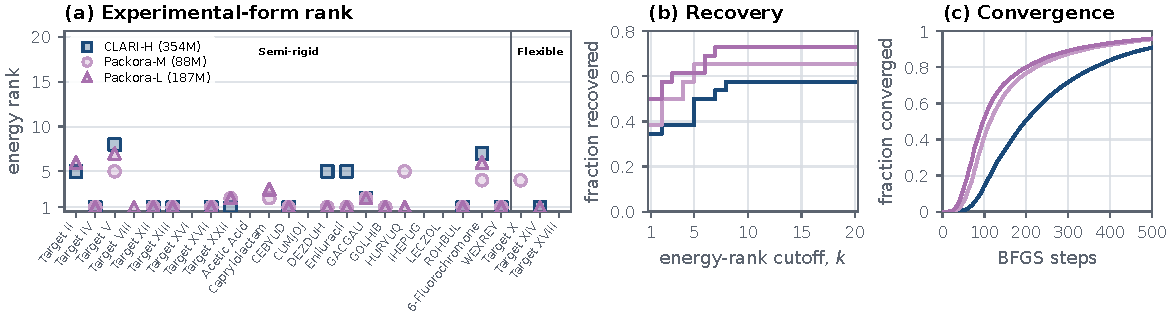
\includegraphics[width=\textwidth]{figures/generated/fig_fastcsp_single_ranking.pdf}
    \caption{\textbf{FastCSP single-polymorph benchmark.}
    We generate 1{,}000 candidates for each of the 26 targets, relax them with
    UMA-S-1.2~\citep{wood2025family}, and rank them by increasing energy.
    \textbf{(a)} Best energy rank of the experimental target form for CLARI-H,
    \model{}-M, and \model{}-L; lower is better, with rank 1 denoting the predicted
    minimum-energy structure. \model{}-L and \model{}-M recover 19 and 17 targets
    within the top 20, respectively, compared with 15 for CLARI-H.
    \textbf{(b)} Fraction of targets recovered by energy-rank cutoff $k$; \model{}
    achieves higher recovery across cutoffs. \textbf{(c)} Cumulative fraction of the
    generated candidates converged by BFGS step; \model{} candidates converge faster
    throughout relaxation. Relaxing all candidates on eight NVIDIA H200 GPUs takes
    16.8, 11.4, and 10.2~h for CLARI-H, \model{}-M, and \model{}-L, respectively.}
    \label{fig:fastcsp-single-ranking}
\end{figure}



\begin{table}[t]
\centering
\caption{\textbf{Experimental-form recovery on FastCSP single-polymorph benchmark.}
We generate 1{,}000 candidates for each of the 26 targets, relax them with
UMA-S-1.2~\citep{wood2025family}, and rank the relaxed structures by increasing
energy. Recovered denotes the fraction of targets with an
experimental-form match at any rank, while Top-$k$ denotes the fraction whose
best match appears within the top $k$ ranks. Mean rank is computed over recovered
targets only, with lower values indicating better ranking. \textbf{Bold} marks
the best result. \model{} achieves both higher recovery across rank cutoffs and
lower experimental-form ranks.}
\label{tab:fastcsp-single-ranking}
\begin{tabular}{lccccc}
\toprule
Method & Recovered $\uparrow$ & Top-1 $\uparrow$ & Top-5 $\uparrow$
& Top-20 $\uparrow$ & Mean rank $\downarrow$ \\
\midrule
CLARI-H & 16/26 & 9/26 & 13/26 & 15/26 & 4.25 \\
\rowcolor{mfTealFill}
\model{}-M & 17/26 & 10/26 & \textbf{17/26} & 17/26 & \textbf{2.00} \\
\rowcolor{mfTealFill}
\model{}-L & \textbf{19/26} & \textbf{13/26} & 16/26 & \textbf{19/26} & 2.05 \\
\bottomrule
\end{tabular}
\end{table}


\textbf{Multi-polymorph results.}
The advantage remains in the multi-polymorph setting. \model{}-M and \model{}-L
recover 19 and 21 of the 29 forms, respectively, compared with 18 for CLARI-H,
and reduce the mean recovered rank from 102.17 to 47.11 and 54.62
(\Cref{tab:fastcsp-multi-ranking,fig:fastcsp-multi-ranking}). Also,
both \model{} variants recover at least one polymorph for all 8 of 8 systems,
whereas CLARI-H recovers 7. Relaxation is also faster: after 100 BFGS steps,
41.4\% and 57.3\% of \model{}-M and \model{}-L candidates have converged,
compared with 13.0\% for CLARI-H. Total relaxation takes 10.6~h and 8.9~h,
respectively, versus 16.8~h for CLARI-H on eight NVIDIA H200 GPUs. Per-form
ranks and $\mathrm{RMSD}_{30}$ values are reported in
\Cref{app:structure-ranking-results}.


\begin{figure}[t]
  \centering
  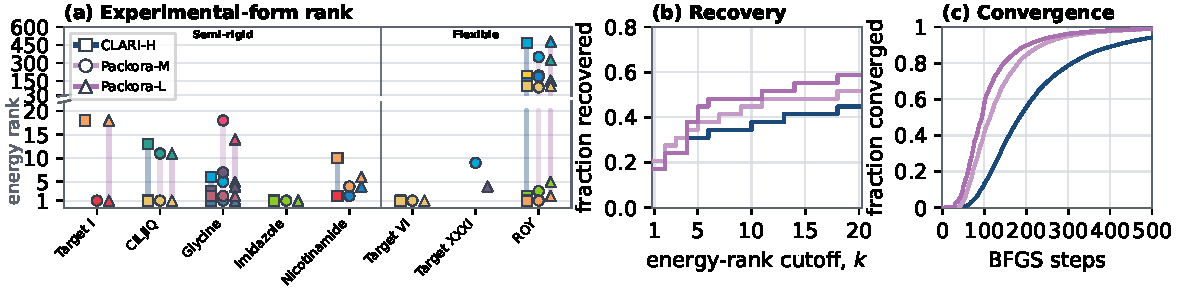
\includegraphics[width=\textwidth]{figures/generated/fig_fastcsp_multi_ranking.pdf}
  \caption{\textbf{FastCSP multi-polymorph benchmark.}
    We generate 1{,}000 candidates for each of the 29 target structures
    across eight systems, relax them with
    UMA-S-1.2~\citep{wood2025family}, and rank them by increasing energy within
    each system. \textbf{(a)} Best energy rank of each of the 29 polymorphs
    for CLARI-H, \model{}-M, and \model{}-L; lower is better, with rank
    1 denoting the predicted minimum-energy structure. Marker color identifies
    the polymorph across systems. \model{}-L and \model{}-M recover
    21 and 19 polymorphs, respectively,
    compared with 18 for CLARI-H. \textbf{(b)} Fraction of
    polymorphs recovered by energy-rank cutoff $k$; \model{} achieves higher
    recovery across cutoffs. \textbf{(c)} Cumulative fraction of the generated candidates converged by BFGS step; \model{} candidates converge faster throughout relaxation.
    Relaxing all candidates on eight NVIDIA H200 GPUs takes 16.8, 10.6, and
    8.9~h for CLARI-H, \model{}-M, and \model{}-L, respectively.}
  \label{fig:fastcsp-multi-ranking}
\end{figure}



\begin{table}[t]
\centering
\caption{\textbf{Experimental-form recovery on FastCSP multiple-polymorph benchmark.}
We generate 1{,}000 candidates for each of the 29 targets, relax them with
UMA-S-1.2~\citep{wood2025family}, and rank the relaxed structures by increasing
energy. Recovered denotes the fraction of targets with an
experimental-form match at any rank, while Top-$k$ denotes the fraction whose
best match appears within the top $k$ ranks. Mean rank is computed over recovered
targets only, with lower values indicating better ranking. \textbf{Bold} marks
the best result. \model{} achieves both higher recovery across rank cutoffs and
lower experimental-form ranks.}
\label{tab:fastcsp-multi-ranking}
\begin{tabular}{lccccc}
\toprule
Method & Recovered $\uparrow$ & Top-1 $\uparrow$ & Top-5 $\uparrow$
& Top-20 $\uparrow$ & Mean rank $\downarrow$ \\
\midrule
CLARI-H & 18/29 & 5/29 & 9/29 & 13/29 & 102.17 \\
\rowcolor{mfTealFill}
\model{}-M & 19/29 & \textbf{6/29} & 11/29 & 15/29 & \textbf{47.11} \\
\rowcolor{mfTealFill}
\model{}-L & \textbf{21/29} & 5/29 & \textbf{13/29} & \textbf{17/29} & 54.62 \\
\bottomrule
\end{tabular}
\end{table}

